\chapter{Results and Analysis}
\label{Chapter:Results}

Tables and figures are handled well by \LaTeX . 

\section{Tables}

Tables can be generated using the tabular environment. To make it possible to reference them, include a caption, and automatically populate the list of tables, wrap this in the table environment.

\begin{table}[h!]
    \caption[Relevant Nuclear Constants]{Relevant nuclear constants \cite{Lamarsh}.}
    \centering\begin{tabular}{c|ccc}
                   & $\gamma \;(\%)$ & $\lambda \; (hr^{-1})$ & $\sigma \; (Mb)$ \\ \hline
        \I  & 6.39            & 0.1035                 & -                \\
        \Xe & 0.237           & 0.0753                 & 2.65
    \end{tabular}
    \label{params}
\end{table}

The caption contains two arguments. The first is wrapped in square brackets and is the "short" version that will populate in the List of Tables. The second is the "long" version, wrapped in curly braces, that will populate above the table. Table \ref{params} has 4 columns, each of which has centered data, with a vertical line after the first column. This is specified by the argument \verb={c|ccc}= after \verb=\begin{tabular}=. Columns are delimited by \& and rows are delimited by \verb=\\=. The label should come after \verb=\end{tabular}= so the compiler doesn't get confused.

\section{Figures}
The figure environment can be used to load in various images and other figures. Like with the table environment, you can develop a label to reference the figure in text, and both a short version and long version of the caption. This is handy to keep your List of Figures tidy while allowing for very descriptive captions under the figure.

\newpage

\subsection{Static Images}
These are included using the \verb=\includegraphics[options]{name}= command. There is a lot more information on the internet, including Dr. Trefor's videos. Figure \ref{BC} is an example. The argument after the \verb=\begin{figure}= is used to position the figure.

\begin{figure}[h!]
    \centering
    \includegraphics[width=0.25\textwidth]{BC}
    \caption[Big Chungus.]{A humorous image of an overweight Buggs Bunny, often referred to as `Big Chungus'.}
    \label{BC}
\end{figure}

\subsection{User Generated Drawings}

Tikz is a package that allows you to make very nice drawings right in \LaTeX \;. Dr. Trefor has a tutorial. The learning curve is steep, and honestly is more difficult to use than GUI sandbox based drawing application, but it has the benefit of being able to keep typeface formatting very consistent. See how nice the equations look in Figure \ref{strip}? Try doing that in MS Paint. 

\begin{figure}[h!]\centering
    

\begin{tikzpicture}
\draw[green, very thick] (-1,-1) rectangle (1,1);
\filldraw[green!10] (-1,-1) rectangle (1,1);
%Bottom
\draw[->] (0,-2)--(0,-1);
\draw node at (-0.15,-2.15) {\small{$c_{He}^{in} = 0$}};
%Top
\draw[->] (0,1)--(0,2);
\draw node at (0.15,2.15) {\small{$c_{He}^{out} = \nicefrac{c_{salt}^{out}}{H^*}$}};
%Left
\draw[->] (-2.75,0)--(-1,0);
\draw node at (-1.0,0.5) [anchor=east]{\small{$c_{salt}^{in} = Xe(t)$}} ;
%Right
\draw[->] (1,0)--(4,0);
\draw node at (1.0,0.5) [anchor = west]{\small{$c_{salt}^{out} = c_{salt}^{in}-c_{He}^{out}\frac{\dot{V}_{He}}{\dot{V}_{salt}}$}};
\end{tikzpicture}

    \caption{Schematic Drawing of Xenon Stripping Module} 
    \label{strip}
\end{figure}

\newpage
\subsection{Animations}
The graphicx package cannot accept .gif files, so the animate package can be used as a proxy. You will need each frame to be an individual .png, but this allows you to stack images over one another, which can give a time component to 2-D plots, or allow you to look at multiple planes of a drawing in a single figure. You will need to open the file in a proper PDF viewer like Adobe - web browsers and PDF previewers found in Overleaf, Atom, VSCode, etc. cannot handle this powerful functionality. I'm not sure if this functionality is allowed in the actual thesis submission, but it can be useful in presentations or meetings. Figure \ref{Bateman} is a visualization of the Bateman equations  causing the xenon spike following the shutdown of a nuclear reactor. It loops through bar-200 to bar-248 at 2 frames per second. You can also step through frame by frame using the arrow controls. Note that feature can cause compile times to be very long so you may wish to comment it out. 

\begin{figure}[h!]
    \centering
    \animategraphics[width=0.60\textwidth, controls]{2}{scram/bar-}{200}{248}
    \caption{Nuclide Concentration Rates of Change - Reactor Scram}
    \label{Bateman}
\end{figure}